\chapter{Mejoras de las físicas en \textit{WebSim}}
\label{chap:motor_fisicas} 
A lo largo de este capítulo se va a explicar la modificación que se ha realizado en el funcionamiento de las físicas de los robots utilizados en \textit{Kibotics WebSim}. Previamente al cambio, los robots se desplazaban gracias a la imposición de una posición concreta cada 50 ms, sin tener en cuenta velocidades ni aceleraciones en el cómputo. El usuario seleccionaba una velocidad objetivo para un robot y el propio \textit{WebSim} (\textit{Simcore}) se encargaba de realizar los cálculos precisos para determinar la posición a la que debía desplazarse el robot. \newline

El motor de físicas complementario que se ha implementado ha introducido las siguientes mejoras en \textit{WebSim}, que permiten dotar al simulador de unas físicas más realistas tanto visualmente como por el funcionamiento interno de las mismas:

\begin{itemize}
    \item \textbf{Materizalización de la gravedad:} los drones son capaces de volar en un mundo que materialice una gravedad de -9.8. Hasta el momento, los ejercicios de drones se configuraban con gravedad 0 para permitir volar al cuerpo.
    \item \textbf{Materialización del coeficiente de rozamiento:} el desplazamiento de los robots no se realiza por imposición de una posición concreta sino por la aplicación de la fuerza necesaria para alcanzar la velocidad objetivo. De esta forma, entran en juego las fuerzas y las aceleraciones que, tras un ajuste en sus valores, permitirán alcanzar la velocidad objetivo sin necesidad de imponer al robot la posición en la que debería encontrarse en cada momento.
\end{itemize}

\section{Estudios previos}
Antes de abordar la creación del motor de físicas complementario se realizó un estudio del comportamiento de la gravedad, las colisiones y la fricción en \textit{WebSim}. A continuación, se incluye una breve explicación del funcionamiento y las posibilidades que ofrece \textit{A-Frame} para parametrizar estos atributos.

\subsection{Estudio de la gravedad} 
Dado que \textit{WebSim} se basa en la tecnología de \textit{A-Frame}, la gravedad es un parámetro configurable dentro de una escena. Los ficheros de configuración de los escenarios de los ejercicios en formato \textit{JSON} incluyen al principio del código las siguientes líneas que permiten seleccionar el valor deseado para la gravedad.

\begin{verbatim}
                    "scene": {
                        "gravity": -9.8
                    }
\end{verbatim}

Como se ha mencionado anteriormente, previamente al cambio introducido en las físicas, los ficheros de configuración de los ejercicios soportados en la plataforma tenían definida una gravedad con valor 0. Esta configuración era necesaria para conseguir hacer volar a los drones, puesto que con una gravedad de -9.8 cualquier cuerpo sólido de la escena caía hacia abajo como consecuencia de la atracción de la gravedad, por lo que no era posible hacer volar a los robots. Actualmente, todos los ejercicios están simulados con un valor de gravedad de -9.8.  \newline

\subsection{Estudio de las colisiones}
Cualquier cuerpo sólido puede colisionar con otro cuerpo incluído en la escena. Las colisiones pueden tener naturaleza elástica o inélastica dependiendo del valor del coeficiente de restitución de los objetos. El coeficiente de restitución es la media de la conservación de la energía cinética cuando se produce un choque entre partículas. Cuando su valor es 1 el choque es perfectamente elástico y cuando es 0, es perfectamente inelástico. 

\begin{equation}
   Coeficiente \,\, de \,\,restitución = \frac{Velocidad \,\, relativa \,\, tras \,\, la \,\, colisión}{Velocidad \,\, relativa \,\, antes \,\, de \,\, la \,\, colisión}
\end{equation} \newline

\textit{A-Frame} también ofrece la posibilidad de parametrizar el coeficiente de restitución. Este parámetro se puede configurar, al igual que la gravedad, al principio del fichero de configuración de los ejercicios incluyendo el siguiente código.

\begin{verbatim}
                    "scene": {
                        "physics": "restitution: 0.5"
                    }
\end{verbatim}

\subsubsection{Colisiones elásticas}
Se dice que una colisión es elástica cuando, tras el choque, se conserva toda la energía cinética. Esta se transfiere por completo desde el objeto que colisiona hasta el objeto que ha sido colisionado. En la realidad, en todo choque parte de la energía se disipa en calor, por lo que este tipo de colisiones es cosiderada ideal. Visualmente, el efecto que tiene es que el objeto que colisiona se queda parado y el objeto colisionado comienza a moverse a la velocidad que se movía el objeto que colisionó con él. La Figura \ref{fig:elastico} muestra un ejemplo de colisión elástica.

\begin{figure}[h!]
    \centering
    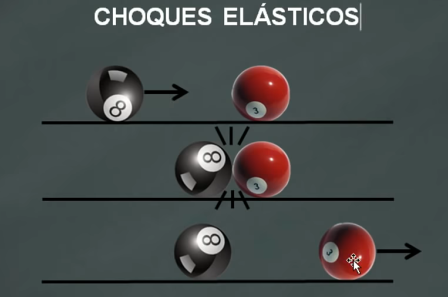
\includegraphics[width=0.7\textwidth, height=0.4\textwidth]{elastico.png}
    \caption{Colisión elástica\footnotemark}
    \label{fig:elastico}
\end{figure}
\footnotetext{https://www.youtube.com/watch?v=b9iOIr5DYj8}


\subsubsection{Colisiones inelásticas}
Por otro lado, cuando se produce una colisión inelástica el objeto que colisiona continúa teniendo parte de la energía cinética, otra parte se transfiere al objeto que ha sido colisionado y la parte restante se disipa en forma de calor. En este tipo de choques el efecto visual es que tanto el objeto que colisiona como el objeto colisionado avanzan a la misma velocidad tras la colisión. La Figura \ref{fig:inelastico} muestra un ejemplo de colisión inelástica.

\begin{figure}[h!]
    \centering
    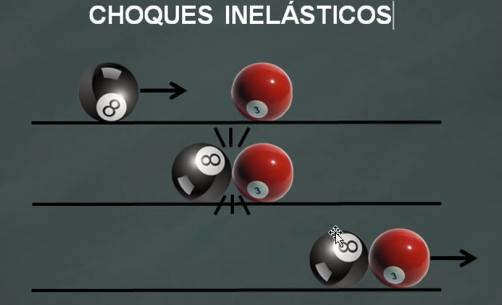
\includegraphics[width=0.7\textwidth, height=0.4\textwidth]{inelasticos.png}
    \caption{Colisión inelástica\footnotemark}
    \label{fig:inelastico}
\end{figure}
\footnotetext{\textit{Ibidem}}

\subsubsection{Pruebas de las colisiones}
Se han realizado pruebas de colisiones en tres escenarios diferentes variando el valor del coeficiente de restitución y la masa de los objetos. Los escenarios utilizados han sido los siguientes:

\begin{itemize}
    \item \textbf{Escenario 1:} dos pelotas cayendo por dos rampas.
    \item \textbf{Escenario 2:} una pelota fija en el suelo y otra cayendo por una rampa.
    \item \textbf{Escenario 3:} una pelota cae por una rampa y colisiona con una pared.
\end{itemize}

\begin{figure}[!h]
  \begin{subfigure}[b]{0.3\textwidth}
    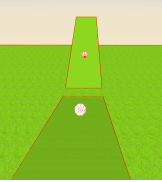
\includegraphics[width=\textwidth, height=\textwidth]{colision1.png}
    \caption{Escenario 1}
  \end{subfigure}
  \hfill
  \begin{subfigure}[b]{0.3\textwidth}
    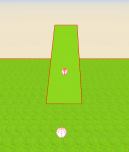
\includegraphics[width=\textwidth, height=\textwidth]{colision2.png}
    \caption{Escenario 2}
  \end{subfigure}
    \hfill
  \begin{subfigure}[b]{0.3\textwidth}
    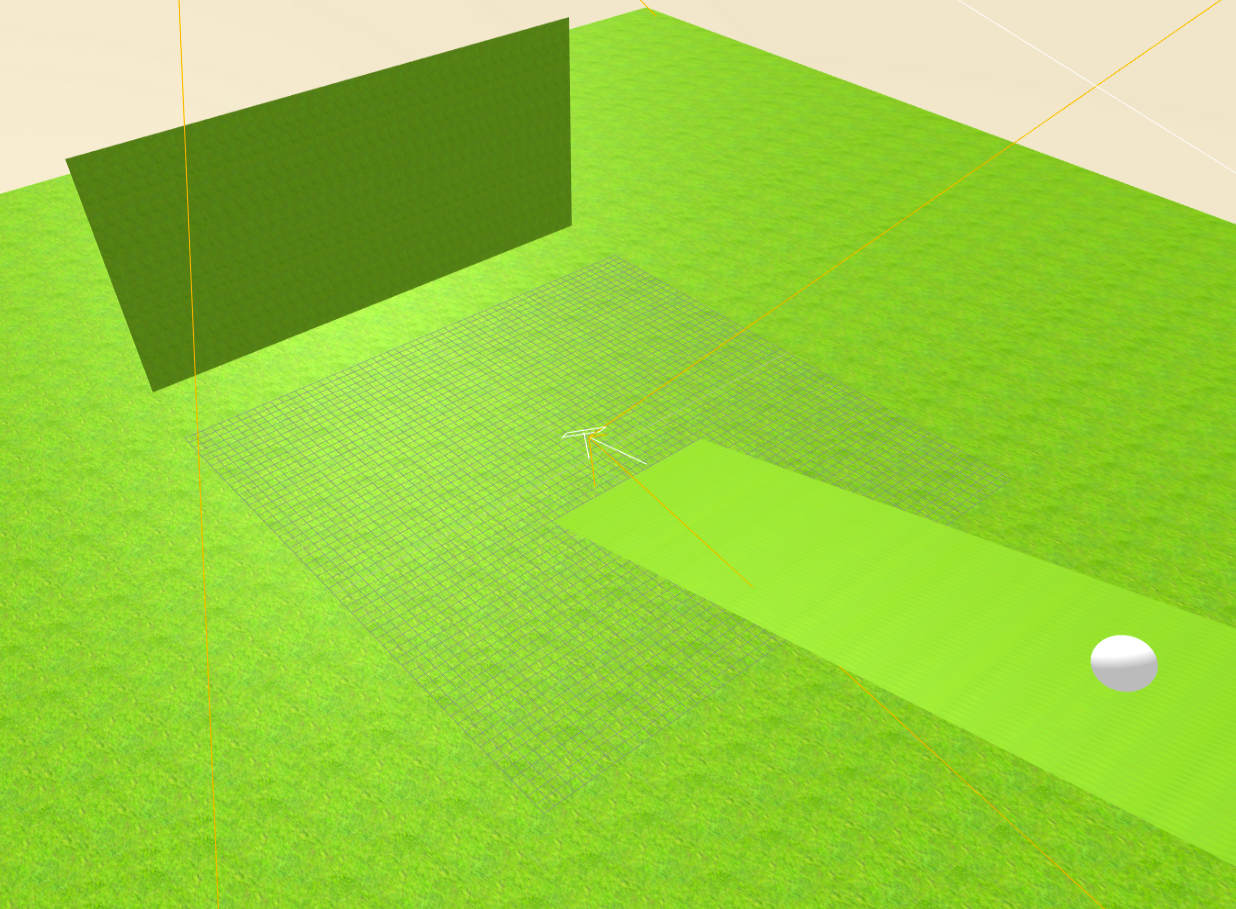
\includegraphics[width=\textwidth, height=\textwidth]{colision3.png}
    \caption{Escenario 3}
  \end{subfigure}
  \caption{Escenarios de prueba de las colisiones de \textit{A-Frame}}
 \end{figure}

Los resultados obtenidos durante las pruebas se detallan en los Cuadros \ref{fig:col-escenario1}, \ref{fig:col-escenario2} y \ref{fig:col-escenario3}.
\begin{table}[]
\centering
 \resizebox{1.1\textwidth}{!}{  
\begin{tabular}{cc}
\hline
\multicolumn{1}{|c|}{\textbf{}}                 & \multicolumn{1}{c|}{\textbf{Misma masa}}                                                                                                                                    \\ \hline
\multicolumn{1}{|c|}{\textbf{Restituion = 0}}   & \multicolumn{1}{c|}{No hay rebote}                                                                                                                  \\ \hline
\multicolumn{1}{|c|}{\textbf{Restituion = 0.4}} & \multicolumn{1}{c|}{Sí hay rebote}                                                                         \\ \hline
\multicolumn{1}{|c|}{\textbf{Restituion = 1}}   & \multicolumn{1}{c|}{La pelota rebota al entrar en contacto con cualquier superfice de la escena}                                                                           \\ \hline
\multicolumn{1}{l}{}                            & \multicolumn{1}{l}{}                                                                                                                                                        \\ \hline
\multicolumn{1}{|l|}{}                          & \multicolumn{1}{c|}{\textbf{Diferente masa}}                                                                                                                                \\ \hline
\multicolumn{1}{|c|}{\textbf{Restituion = 0}}   & \multicolumn{1}{c|}{Las dos pelotas avanzan pegadas en la dirección de la de mayor masa}                                                                                    \\ \hline
\multicolumn{1}{|c|}{\textbf{Restituion = 0.4}} & \multicolumn{1}{c|}{La pelota más pesada hace cambiar la dirección del movimiento de la más ligera, que se desplaza a mayor velocidad} \\ \hline
\multicolumn{1}{|c|}{\textbf{Restituion = 1}}   & \multicolumn{1}{c|}{Las dos pelotas avanzan separadas en la dirección de la de mayor masa. La pelota de menor masa coge mayor velocidad}                                    \\ \hline
\end{tabular}
}
\caption{Resultados de las colisiones obtenidos con el escenario 1}
\label{fig:col-escenario1}
\end{table}

                                                                                                   
\begin{table}[]
\centering
 \resizebox{1.1\textwidth}{!}{  
\begin{tabular}{cc}
\hline
\multicolumn{1}{|c|}{\textbf{}}                 & \multicolumn{1}{c|}{\textbf{Misma masa}}                                                                                                                                                                                                                                                                                                                                                                               \\ \hline
\multicolumn{1}{|c|}{\textbf{Restituion = 0}}   & \multicolumn{1}{c|}{Ambas pelotas avanzan pegadas a la misma velocidad}                                                                                                                                                                                                                                                                              \\ \hline
\multicolumn{1}{|c|}{\textbf{Restituion = 0.4}} & \multicolumn{1}{c|}{La pelota que permanecía en el suelo se mueve más rápido que la que cayó por la rampa. No avanzan pegadas}                                                                                                                                                                                                                                                                           \\ \hline
\multicolumn{1}{|c|}{\textbf{Restituion = 1}}   & \multicolumn{1}{c|}{La pelota rebota al entrar en contacto con cualquier superfice de la escena}                                                                                                                                                                                                                                                                                                                      \\ \hline
\multicolumn{1}{l}{}                            & \multicolumn{1}{l}{}                                                                                                                                                                                                                                                                                                                                                                                                   \\ \hline
\multicolumn{1}{|l|}{}                          & \multicolumn{1}{c|}{\textbf{Diferente masa}}                                                                                                                                                                                                                                                                                                                                                                           \\ \hline
\multicolumn{1}{|c|}{\textbf{Restituion = 0}}   & \multicolumn{1}{l|}{\begin{tabular}[c]{@{}l@{}}- Masa pelota rampa < Masa pelota suelo: ambas pelotas se quedan juntas y paradas\\ - Masa pelota rampa > Masa pelota suelo: ambas pelotas avanzan hacia adelante juntas y a la misma velocidad\end{tabular}}                                                        \\ \hline
\multicolumn{1}{|c|}{\textbf{Restituion = 0.4}} & \multicolumn{1}{l|}{\begin{tabular}[c]{@{}l@{}}- Masa pelota rampa < Masa pelota suelo: la pelota que ha caído por la rampa rebota hacia arriba\\ - Masa pelota rampa > Masa pelota suelo: la pelota que estaba en reposo avanza con más velocidad \\ que la que cayó por la rampa\end{tabular}} \\ \hline
\multicolumn{1}{|c|}{\textbf{Restituion = 1}}   & \multicolumn{1}{c|}{La pelota rebota al entrar en contacto con cualquier superfice de la escena}                                                                                                                                                                                                                                                                                                                      \\ \hline
\end{tabular}
}
\caption{Resultados de las colisiones obtenidos con el escenario 2}
\label{fig:col-escenario2}
\end{table}

\begin{table}[]
\centering
 \resizebox{1.1\textwidth}{!}{  
\begin{tabular}{cc}
\hline
\multicolumn{1}{|c|}{\textbf{}}                 & \multicolumn{1}{c|}{\textbf{Misma masa}}                                                                                       \\ \hline
\multicolumn{1}{|c|}{\textbf{Restituion = 0}}   & \multicolumn{1}{c|}{Permanece junto a la pared, sin rebote} \\ \hline
\multicolumn{1}{|c|}{\textbf{Restituion = 0.4}} & \multicolumn{1}{c|}{Sí hay rebote}                                                                       \\ \hline
\multicolumn{1}{|c|}{\textbf{Restituion = 1}}   & \multicolumn{1}{c|}{El rebote es muy elevado y vuelve a subir la rampa pŕacticamente a la misma velocidad que la bajó}         \\ \hline
                                                &                                                                                                                                \\ \hline
\multicolumn{1}{|c|}{}                          & \multicolumn{1}{c|}{\textbf{Diferente masa}}                                                                                   \\ \hline
\multicolumn{1}{|c|}{\textbf{Restituion = 0}}   & \multicolumn{1}{c|}{Permanece junto a la pared, sin rebote}                                                                            \\ \hline
\multicolumn{1}{|c|}{\textbf{Restituion = 0.4}} & \multicolumn{1}{c|}{Cuanto más pequeña es la masa, más grande es el rebote}                                                                            \\ \hline
\multicolumn{1}{|c|}{\textbf{Restituion = 1}}   & \multicolumn{1}{c|}{Cuanto más pequeña es la masa, más grande es el rebote}                                                                            \\ \hline
\end{tabular}
}
\caption{Resultados de las colisiones obtenidos con el escenario 3}
\label{fig:col-escenario3}
\end{table}

 
\subsection{Estudio de la fricción}
Cualquier cuerpo dinámico de una escena de \textit{A-Frame} presenta una fuerza de rozamiento que se opone al movimiento. Este parámetro, al igual que los dos anteriores, es configurable dentro de la propia escena introduciendo al principio del fichero de configuración las siguientes líneas de código. Gracias a este atributo un objeto posee rozamiento estático y dinámico.

\begin{verbatim}
                    "scene": {
                        "physics": "friction: 0.5"
                    }
\end{verbatim}

\subsubsection{Rozamiento estático}
Dos superficies rígidas en reposo no se desplazan una respecto a la otra siempre y cuando la fuerza paralela al plano tangente sea suficientemente pequeña. Cuando el coeficiente de rozamiento estático de una superifice es excesivamente pequeño, los objetos que se encuentran sobre esa superficie no pueden permanecer en reposo. Una forma de calcular el coeficiente de rozamiento estático es hacer variar la inclinación de una rampa. Cuando se alcanza un ángulo de inclinación con el cual el cuerpo comienza a descender se dice que se ha llegado al ańgulo critico. A partir del ángulo crítico se puede obtener el coeficiente de rozamiento estático gracias a la siguiente igualdad:

\begin{equation}
    tan(angulo \,\, crítico) = coeficiente \,\, de \,\, rozamiento \,\, estático \,\,
\end{equation}

\subsubsection{Rozamiento dinámico}
Cuando dos superficies son puestas en contacto, el movimiento de una respecto a la otra genera fuerzas tangenciales llamadas fuerzas de fricción o rozamiento, las cuales tienen sentido opuesto al movimiento. La magnitud de esta fuerza depende del coeficiente de rozamiento dinámico. En \textit{A-Frame}, el rozamiento dinámico se puede configurar utilizando los atributos \textit{linear-damping y angular-damping} a nivel de objeto, además del atributo \textit{friction} a nivel de escena como se ha mencionado anteriormente. Esos parámetros se pueden parametrizar añadiendo las siguientes líneas de código en los ficheros de configuración.

\begin{verbatim}
               attr": {
                        "static-body": {
                            "linearDamping":1.2,
                            "angularDamping":1.2
                        }
\end{verbatim}

\subsubsection{Pruebas de la fricción}
Se han realizado diferentes pruebas de fricción colocando un objeto en una rampa y variando la inclinación de la misma. Los resultados obtenidos han sido los siguientes:
\begin{itemize}
    \item \textbf{Prueba del rozamiento estático: } se coloca un objeto sobre una rampa y se procede a la variación de la inclinación de la misma. El objeto permanece en la misma posición hasta que se alcanza un ángulo de inclinación tan elevado que el cuerpo comienza a descender (ángulo crítico). Si se configura el atributo \textit{friction} con un valor más elevado, el ángulo crítico se alcanza más tarde, es decir, es mayor.
    \item \textbf{Prueba del rozamiento dinámico: } se mantiene fija la inclinación de la rampa y se varía el valor de los atributos \textit{friction, linear-damping y angular-damping}. Con unos valores elevados de esos tres parámetros, los robots no son capaces de subir la rampa. Sin embargo, a medida que se va reduciendo el valor de los parámetros los robots comienzan a poder subir la rampa y cada vez lo hacen con mayor facilidad.
\end{itemize}

\section{Motor de físicas complementario}
El motor de físicas complementario que se ha implementado basa su funcionamiento en un modelo de controlador PD (controlador proporcional derivativo) con el cual se determina la fuerza necesaria a aplicar al robot para que este se mueva según las órdenes dadas por el usuario.\newline

El controlador PD es una variante del controlador PID (controlador proporcional, integral y derivativo) que no incluye la componente integral. Se trata de un controlador por realimentación que calcula la desviación o error entre una medida y el valor que se desea obtener. Cada componente tiene una utilidad diferente y depende de distintos factores:
\begin{itemize}
    \item \textbf{Componente proporcional: }depende del error actual y su función es minimizar el error del sistema.
    \item \textbf{Componente derivativa: }depende de los errores pasados y permite estabilizar el sitema reduciendo la oscilación del valor de salida.
    \item \textbf{Componente integral: }es una predicción de los errores futuros y se utiliza cuando el componente derivativo no consigue reducir el error del sistema. Su uso es complejo ya que puede producir la desastibilización del sistema.
\end{itemize}

\begin{figure}[h!]
    \centering
    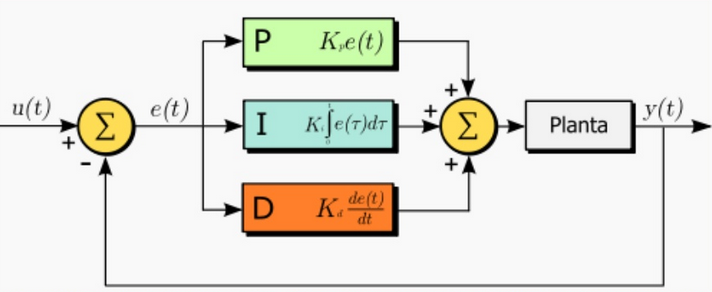
\includegraphics[scale=0.7]{pid.png}
    \caption{Controlador PID \footnotemark}
    \label{fig:pid}
\end{figure}
\footnotetext{https://es.slideshare.net/quasar.0360.7912/sintonizacion-de-controladores-pid}

Mediante un sencillo algoritmo basado en la suma de estos tres componentes, el controlador es capaz de ajustar su salida a un valor de referencia. Además, el modelo incluye tres constantes que se emplean para ponderar los componentes anteriores. En este caso sólo se van a tener en cuenta los componentes proporcionales y derivativos puesto que se van a implementar controladores PD ya que el error del sistema no es excesivamente elevado.\newline 

\begin{figure}[h!]
    \centering
    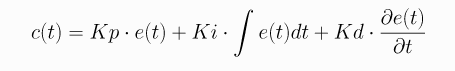
\includegraphics[scale=0.6]{pid_form.png}
    \label{fig:pid_form}
\end{figure}

Antes de implementar los controladores PD en los que se basa el motor de físicas complementario, el movimiento de los robots se recreaba mediante la actualización de su posición cada 50 ms. No entraban en juego ni velocidades ni aceleraciones ni fuerzas. La siguiente función es la que se ha estado utilizando hasta el momento para actualizar las posiciones y hacer moverse a los robots en \textit{WebSim}.

\small{
\begin{verbatim} 
    updatePosition(rotation, velocity, robotPos) {
        if(simEnabled){
            let x = velocity.x / 10 * Math.cos(rotation.y * Math.PI / 180);
            let z = velocity.x / 10 * Math.sin(-rotation.y * Math.PI / 180);
            let y = (velocity.y / 10);
            robotPos.x += x;
            robotPos.z += z;
            robotPos.y += y;
        }
        return robotPos;
}
\end{verbatim}
}

\normalsize
El motor de físicas complementario calcula la fuerza que se debe aplicar a cada robot cada 20 ms gracias a la utilización de un \textit{timeout} que ejecuta los controladores de manera cíclica. Para conseguir una correcta combinación entre el motor complementario y el motor de \textit{CANNON} ha sido necesario calcular cuántas veces actualiza \textit{CANNON} las velocidades y posiciones de un objeto en 20 ms. Este cómputo se ha podido realizar gracias a la creación de un nuevo componente auxiliar que hace incrementar un contador en uno por cada tick de renderizado que ejecuta \textit{A-Frame}. \newline

La siguiente línea de código es la que permite que el nuevo motor complementario se ejecute cada 20 ms.
\small {
\begin{verbatim}
            setTimeout(this.auxiliaryPhysics.bind(this), 20);
\end{verbatim}
}
\normalsize
Las variables y funciones que se han añadido al código original para llevar a cabo la implementación han sido las que se incluyen a continuación. Las funciones \textit{tickCounter, getTickCounter y setTickCounter} se han utilizado para contabilizar el número de veces que se ejecuta el motor de \textit{CANNON} entre dos iteraciones del motor complementario. Por otro lado, el resto de variables se han creado dentro de una clase para que puedan asociarse a un único robot. De esta manera, se evitan los problemas de sobreescritura de variables en los ejercicios multirobot.

\small {
\begin{verbatim}
                export var tickCounter = 0;
                
                export function getTickCounter() {
                    return tickCounter;
                }
                export function setTickCounter(value) {
                    tickCounter = value;
                }
\end{verbatim}
}


\small {
\begin{verbatim}
                export class RobotI {
                    constructor(robotId) {
                        this.errorY = 0;
                        this.errorXZ = 0;
                        this.errorW = 0;
                        this.errorActualY = 0;
                        this.errorActualXZ = 0;
                        this.errorActualW = 0;
                        this.derivadaErrorY = 0;
                        this.derivadaErrorXZ = 0;
                        this.derivadaErrorW = 0;
                        this.forcePD = 0;
                        this.accelerationPD = 0;
                        this.commandedVelocityY = 0;
                        this.commandedVelocityXZ = 0;
                        this.commandedVelocityW = 0;
                        this.accelerationPDY = 0;
                        this.accelerationPDXZ = 0;
                        this.accelerationPDW = 0;
                        this.resultVelocity = 0;
                        this.refPos = 0;
                        this.init = true;
                        this.stop = true;
                        this.motorIterations = 0;
                }
\end{verbatim}
}
\normalsize
Para crear el nuevo componente se han utilizado las herramientas que ofrece \textit{A-Frame} para el registro de nuevos componentes. La siguiente línea de código realiza el registro del nuevo componente auxiliar que se utiliza para contabilizar las iteraciones de \textit{CANNON}. A continuación, también se ha incluido el código del tick del nuevo componente registrado.

\small {
\begin{verbatim}
            /* Registro del nuevo componente */
            AFRAME.registerComponent("iterations", iterationsObj);
            
            /* Función tick del componente "iterations" */
            export var iterationsObj = {
                schema: {
                  count: { type: 'number', default: 0 },
                  position: { "x":0, "y":0, "z":0}
                },
                tick: function(){
                  setTickCounter(getTickCounter() + 1);
                  console.log('Tick de renderizado de A-FRAME');
                }
              }
            }
\end{verbatim}
}

\subsection{Mejoras en el movimiento lineal}
\subsubsection{Eje vertical}
\normalsize
Estas mejoras afectan a los ejercicios para drones que incluye el entorno \textit{Kibotics}. Para controlar el movimiento vertical de los robots se han creado dos controladores PD de la fuerza a aplicar. Uno de ellos tiene como entrada la posición del robot y, el otro, la velocidad. Con ellos se consigue alcanzar la velocidad objetivo que fija el usuario para un robot y se mantiene fija la altura durante vuelo de los drones. \newline

Por un lado, el controlador en posición se utiliza cuando el robot se encuentra en suspensión. El controlador toma como entrada la posición de renferencia del eje Y en la que debe permanecer el robot y genera como salida la fuerza a aplicar para mantener dicha posición. Por otro lado, el controlador en velocidad toma como entrada la velocidad objetivo que se desea alcanza y su salida es, de la misma forma que con el controlador anterior, la fuerza necesaria para alcanzar dicha velocidad. \newline 

La Figura \ref{fig:pd_pos} muestra la salida de este controlador cuando la posición de referencia es 9,75 m Y la Figura \ref{fig:pd_velY} muestra la salida de este controlador cuando la velocidad de referencia es 2 ms^{-1}.

\begin{figure}[h!]
    \centering
    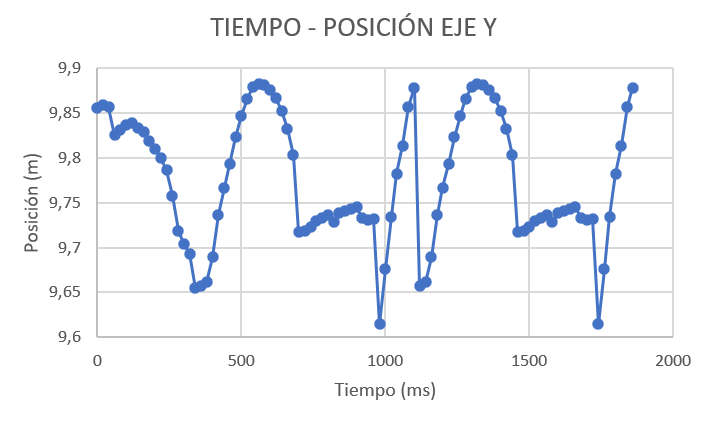
\includegraphics[scale=1]{tiempo - posicion eje Y.PNG}
    \caption{Controlador PD en posición eje Y}
    \label{fig:pd_pos}
\end{figure}

\begin{figure}[h!]
    \centering
    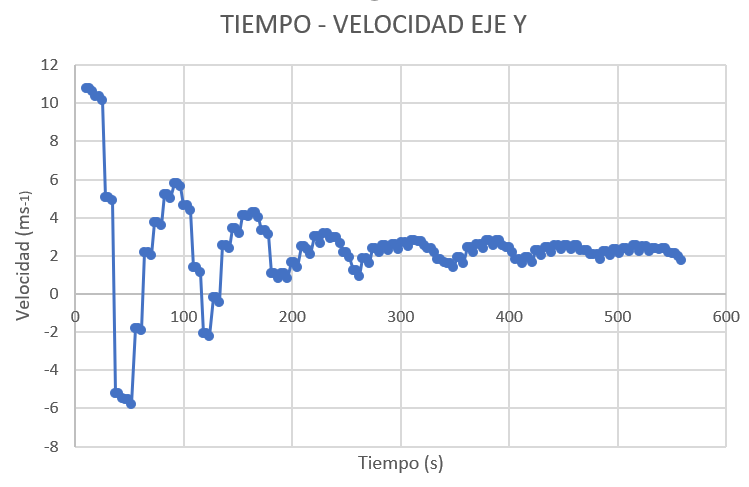
\includegraphics[scale=0.9]{VELOCIDAD EJE Y.PNG}
    \caption{Controlador PD en velocidad eje Y}
    \label{fig:pd_velY}
\end{figure}

A continuación se incluye el código de ambos controladores junto a algunos comentarios que aclaran su funcionamiento.

\footnotesize {
\begin{verbatim}
/*Actualización del contador de iteraciones*/
this.motorIterations = getTickCounter(); 
           
/* Si la velocidad de vuelo objetivo es 0: */
if ((this.velocity.y <= 0.0001) || (this.velocity.y <= -0.0001)){
    if (this.init == true) {
    /* Si el movimiento aún no ha comenzado la aceleración debe ser 0 */
        this.accelerationPDY = 0;
    } else { 
    /* Si el movimiento ya ha comenzado: */
	    if (this.stop == true) {
	/* Si se acaba de quedar en suspensión, guardo la posición de referencia */
		  this.refPos = this.robot.body.position.y;
		 }
	/* Entra el controlador PD en posiciones */
        this.stop = false;
		this.accelerationPDY = this.controladorPDVerticalPos();
	}
/* Si la velocidad objetivo no es 0, se ejecuta el controlador PD en velocidades */
} else {
    this.init = false;
    this.stop = true;
    this.accelerationPDY = this.controladorPDVerticalVel();
}
            
/* Se utiliza la aceleración calculada con los controladores para obtener la velocidad 
a aplicar utilizando las fórmulas MRUA y la combinación entre motores */
            
    this.commandedVelocityY = this.robot.body.velocity.y + 
    this.motorIterations*this.accelerationPDY;
    this.robot.body.velocity.set(this.robot.body.velocity.x, this.commandedVelocityY,
    this.robot.body.velocity.z); 
}
\end{verbatim}
}

\footnotesize {
\begin{verbatim}
/* Código del controlador PD en posición */
    controladorPDVerticalVel() {
        /* Definición constantes para el controlador, fuerza máxima y                   aceleración máxima */
        const mass = this.robot.body.mass;
        const kp = 0.45*mass;
        const kd = 0.12*mass;
        const fMax = 1000000;
        const accelerationMax = fMax / mass;

        /* Cálculo del error y derivada del error*/
        this.errorActualY = this.velocity.y - this.robot.body.velocity.y; 
        this.derivadaErrorY = this.errorActualY - this.errorY;
        this.errorY = this.errorActualY;
        
        /* Salida del controlador */
        this.forcePD = kp*this.errorActualY + kd*this.derivadaErrorY;
        
        /* Obtención de la aceleración teniendo en cuenta la masa */
        this.accelerationPD = this.forcePD / mass;

        /* Límite de aceleración aplicable en cada iteración */
        if (Math.abs(this.accelerationPD) > angularAccelerationMax) {
            if (this.accelerationPD > 0) {
                this.accelerationPD = angularAccelerationMax;
            } else {
                this.accelerationPD = - angularAccelerationMax;
            }
        }
        return this.accelerationPD;
    }
    
/* Código del controlador PD en velocidad */
    controladorPDVerticalPos() {
        /* Definición constantes para el controlador, fuerza máxima y                   aceleración máxima */
        const mass = this.robot.body.mass;
        const kp = 0.95*mass;
        const kd = 0.95*mass;
        const fMax = 100000000;
        const accelerationMax = fMax / mass;

        /* Cálculo del error y derivada del error*/
        this.errorActualY = this.refPos - this.robot.body.position.y;
        this.derivadaErrorY = this.errorActualY - this.errorY;
        this.errorY = this.errorActualY;
        
        /* Salida del controlador */
        this.forcePD = kp*this.errorActualY + kd*this.derivadaErrorY;
        
        /* Obtención de la aceleración teniendo en cuenta la masa */
        this.accelerationPD = this.forcePD / mass;

        /* Límite de aceleración aplicable en cada iteración */
        if (Math.abs(this.accelerationPD) > angularAccelerationMax) {
            if (this.accelerationPD > 0) {
                this.accelerationPD = angularAccelerationMax;
            } else {
                this.accelerationPD = - angularAccelerationMax;
            }
        }
        return this.accelerationPD;
    }
}
\end{verbatim}
}

\normalsize
Las mejoras introducidas son tanto a nivel visual como del funcionamiento interno de las físicas. Se ha conseguido un vuelo más fluido y realista y, además, gracias a estos controladores se puede aplicar sobre el drone la fuerza necesaria para superar la fuerza de la gravedad y hacer ascender o descender al robot a la velocidad fijada, evitando así la caída libre de los robots debido a la fuerza de la gravedad.

\subsubsection{Plano horizontal}
Para controlar el movimiento lineal horizontal también se ha implementado un controlador PD en velocidad. Este utiliza la velocidad como parámetro de entrada al controlador y genera como salida la fuerza a aplicar al robot para alcanzar la velocidad de referencia seleccionada. \newline

Gracias a estos controladores se otorga un mayor realismo al movimiento en el plano horizontal, ya que entran en juego las aceleraciones y las fuerzas y se empieza a tener en cuenta otros parámetros de la escena como la fricción. De esta manera, el controlador debe obtener como salida la fuerza necesaria para superar la fuerza de rozamiento de las distintas superficies. Anteriormente, al imponer la posición directamente sobre el objeto, no era necesario tener en cuenta la dinámica de las fuerzas y aceleraciones de los cuerpos, ya que simplemente se imponía la posición del robot mediante una instrucción \textit{set}. \newline

La Figura \ref{fig:pd_velXZ} muestra la salida de este controlador cuando la velocidad de referencia es 2 ms^{-1}.

\begin{figure}[h!]
    \centering
    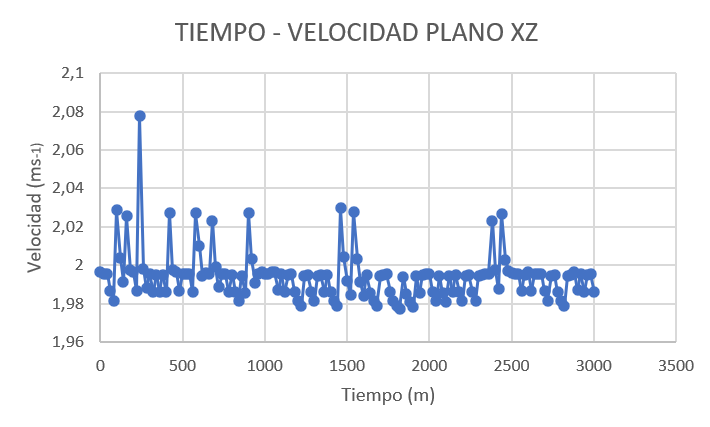
\includegraphics[scale=0.9]{tiempo - velocidad X.PNG}
    \caption{Controlador PD en velocidad eje Y}
    \label{fig:pd_velXZ}
\end{figure}

A continuación se incluye el código del controlador junto a algunos comentarios que aclaran su funcionamiento.

\footnotesize {
\begin{verbatim}
    /* Movimiento en el plano horizontal */
    
/* Velocidad resultante = RaízCuadrada(Vx ² + Vz²)*/
	this.resultVelocity = Math.sqrt(Math.pow(this.robot.body.velocity.x, 2) + 
	Math.pow(this.robot.body.velocity.z, 2));
	
	/* Entra el controlador PD */
	this.accelerationPDXZ = this.controladorPDHorizontal(this.resultVelocity); 
	
	/* Se utiliza la aceleración calculada con los controladores para obtener la velocidad 
a aplicar utilizando las fórmulas MRUA y la combinación entre motores */
	this.commandedVelocityXZ = this.resultVelocity + 
	this.motorIterations*this.accelerationPDXZ;
	let rotation = this.getRotation();
	
	/* La velocidad comandada resultante se descompone en las velocidades Vx y Vz */
	this.robot.body.velocity.set(this.commandedVelocityXZ*Math.cos(rotation.y*Math.PI/180), 
	this.robot.body.velocity.y,this.commandedVelocityXZ*Math.sin(-rotation.y*Math.PI/180));
\end{verbatim}
}

\footnotesize {
\begin{verbatim}
/* Código del controlador PD en velocidad */
    controladorPDHorizontal(resultVelocity) {
    /* Definición constantes para el controlador, fuerza máxima y aceleración máxima */
        const mass = this.robot.body.mass;
        const kp = 0.45*mass;
        const kd = 0.01*mass;
        const fMax = 100000000;
        const accelerationMax = fMax / mass;

        /* Cálculo del error y derivada del error*/
        this.errorActualXZ = this.velocity.x - resultVelocity;
        this.derivadaErrorXZ = this.errorActualXZ - this.errorXZ;
        this.errorXZ = this.errorActualXZ;

        /* Salida del controlador */
        this.forcePD = kp*this.errorActualXZ + kd*this.derivadaErrorXZ;
        
        /* Obtención de la aceleración teniendo en cuenta la masa */
        this.accelerationPD = this.forcePD / mass;

        /* Límite de aceleración aplicable en cada iteración */
        if (Math.abs(this.accelerationPD) > angularAccelerationMax) {
            if (this.accelerationPD > 0) {
                this.accelerationPD = angularAccelerationMax;
            } else {
                this.accelerationPD = - angularAccelerationMax;
            }
        }
        return this.accelerationPD;
    }
\end{verbatim}
}

\normalsize
Como se ha mencionado previamente, la principal mejora que introduce esta implementación es que se empiezana  tener en cuenta aceleraciones y fuerzas, lo que permite la simulación de escenarios muy diversos como podría ser una pista de hielo en la que la fricción es muy reducida y el controlador PD tarda más tiempo en conseguir frenar un objeto tras un movimiento, por ejemplo. La Figura \ref{fig:friccion-acele} muestra la variación en la aceleración necesaria para alcanzar una misma velocidad objetivo con valores de fricción diferentes. Como se puede observar, cuanto mayor es la fricción del escenario mayor es la fuerza a aplicar para superar la fuerza de rozamiento y, por tanto, mayor es la aceleración que se aplica al robot.

\begin{figure}[h!]
    \centering
    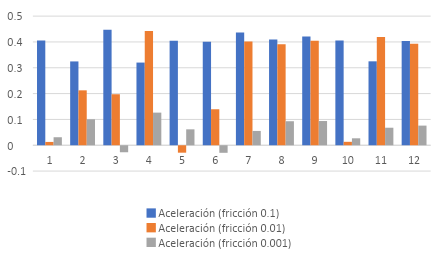
\includegraphics[scale=0.9]{aceleracion-friccion.png}
    \caption{Relación fricción - aceleración}
    \label{fig:friccion-acele}
\end{figure}


\subsection{Mejoras en el movimiento angular}
Por último, también se han incluido dos controladores PD para obtener la velocidad angular necesaria para hacer girar a un robot. En este caso ha sido necesaria la definición de las constantes Kp y Kd de manera independiente para robots terrestres y drones. La razón es que en el giro de los robots terrestres entra en juego la fricción y en el de los drones no. En consecuencia es necesario que existan dos controles independientes para obtener una salida fiable en ambos casos. 

La Figura \ref{fig:pd_velang} muestra la salida de este controlador cuando la velocidad de referencia es 2 ms^{-1}.

\begin{figure}[h!]
    \centering
    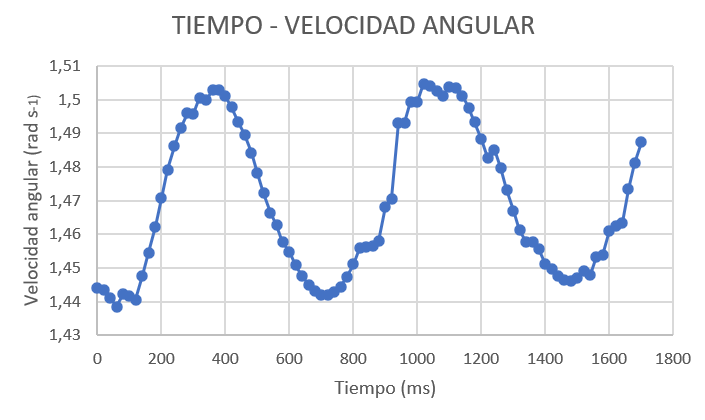
\includegraphics[scale=0.9]{tiempo - velocidad angular.PNG}
    \caption{Controlador PD en velocidad angular}
    \label{fig:pd_velang}
\end{figure}

A continuación se incluye el código del controlador junto a algunos comentarios que aclaran su funcionamiento.

\footnotesize {
\begin{verbatim}
    /* Movimiento angular */
     
    /* Entra el controlador PD angular */              
    this.accelerationPDW = this.controladorPDAngular();
    
    /* Se utiliza la aceleración calculada con el controlador para obtener 
    la velocidad angular a aplicar utilizando las fórmulas MRUA y la 
    combinación entre motores */
    this.commandedVelocityW = this.robot.body.angularVelocity.y + 
    this.motorIterations*this.accelerationPDW;
    this.robot.body.angularVelocity.set(0, this.commandedVelocityW, 0);
    console.log("Velocidad angular: " + this.commandedVelocityW);
    
    /* Código del controlador PD en velocidad angular*/
    controladorPDAngular() {
        /* Definición constantes para el controlador, torque máximo, inercia 
        y aceleración máxima */
        const mass = this.robot.body.mass;
        
        /* Distinción entre robot terrestre o volador. Init es true cuando un 
        robot comienza el vuelo por primera vez */   
        if (this.init == false) {
    	    var kp = 0.6*mass;
    	    var kd = 0.12*mass;
    	    var tMax = 100;
        } else {
    	    var kp = 0.05*mass;
    	    var kd = 0.01*mass;
    	    var tMax = 1;
        }

        const inertia = this.robot.body.inertia.x;
        const angularAccelerationMax = tMax / inertia;

         /* Cálculo del error y derivada del error*/
        this.errorActualW = this.velocity.ay - this.robot.body.angularVelocity.y; 
        this.derivadaErrorW = Math.abs(this.errorW - this.errorActualW);
        this.errorW = this.errorActualW;

        /* Salida del controlador */
        this.forcePD = kp*this.errorActualW + kd*this.derivadaErrorW;
        
        /* Obtención de la aceleración teniendo en cuenta la inercia */
        this.accelerationPD = this.forcePD / inertia;

        /* Límite de aceleración aplicable en cada iteración */
        if (Math.abs(this.accelerationPD) > angularAccelerationMax) {
            if (this.accelerationPD > 0) {
                this.accelerationPD = angularAccelerationMax;
            } else {
                this.accelerationPD = - angularAccelerationMax;
            }
        }
        return this.accelerationPD;
    }
\end{verbatim}
}

\normalsize
La principal mejora que introduce el control en velocidad angular es que los robots no empiezan ni dejan de girar de un instante a otro tal y como ocurría antes. Las aceleraciones que se aplican a los robots gracias al controlador PD hacen que la velocidad angular de giro al principio y al final del movimiento sea más pequeña, ofreciendo al usuario a efectos visuales un movimiento mucho más realista.